
\begin{questions}

% 2.1  % % % % % % % % % % % % % % % % % % % % %
% \setcounter{question}{1}
\question{
Esboce e encontre uma parametrização para a curva ${\cal C}$ dada pela interseção entre o cilindro $x^2 + y^2 = 1$ e o plano $y + z = 2$. Determine a reta tangente a esta curva no ponto $(-1,0,2)$.
}
\begin{solution}

\begin{center}
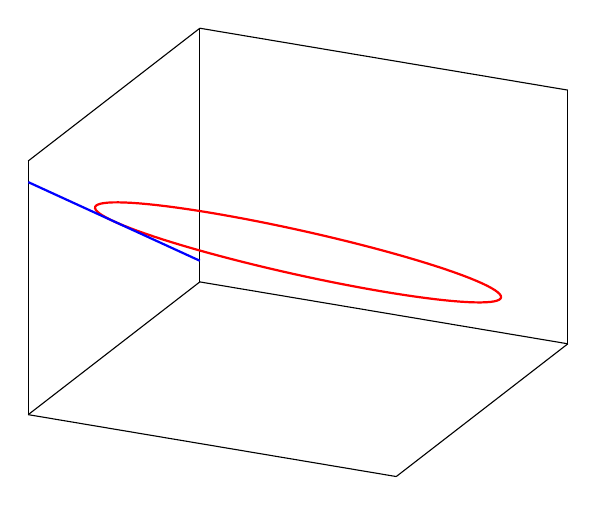
\begin{tikzpicture}
  \begin{axis}[
    xtick      = \empty,
    ytick      = \empty,
    ztick      = \empty
  ]
  \addplot3+ [
    domain     = 0:360,
    samples    = 100,
    samples y  = 0,
    mark       = none,
    thick,
    red,
  ]
  ( {cos(x)}, {sin(x)}, {2-sin(x)} );
  \addplot3+ [
    domain     = -1:1,
    samples    = 100,
    samples y  = 0,
    mark       = none,
    thick,
    blue,
  ]
  ( {-1}, {-x}, {2+x} );
  \end{axis}
\end{tikzpicture}
\end{center}

Uma possível parametrização em $t\in[0,2\pi)$ é
\begin{align*}
    \begin{cases}
        x = \cos t, \\
        y = \sin t, \\
        z = 2 - \sin t.
    \end{cases}
\end{align*}
    Sabemos que $\vec r (t=\pi) = (-1,0,2)$. Assim, um possível vetor diretor da reta tangente é dado por $\dot {\vec r}(t = \pi) = (-\sin(\pi), \cos(\pi), -\cos(\pi)) = (0,-1,1)$. Logo, a reta tangente
    \[\vec s = (-1,0,2) + [(0,-1,1)].\]
\end{solution}

% 2.2 % % % % % % % % % % % % % % % % % % % % %
% \setcounter{question}{2}
\question{
Mostre que a curva dada por 
\[
\vec r(t) = \Big(t \cos t , t \sin t, t \Big), \quad t \in \R,
\]
está contida no cone $z^2 = x^2 + y^2$. Use esta informação para esboçar o traço de $\vec r$.
}

\begin{solution}
    Para mostrar que a curva está contida no cone, basta verificar que a curva satisfaz a equação do cone para todo $t\in\R$, ou seja, $t^2 = (t \cos t)^2 + (t \sin t)^2 \quad \forall t\in\R$.
    
\begin{center}
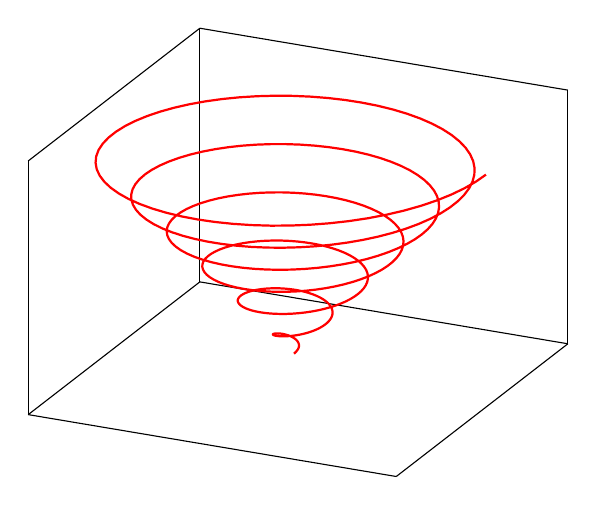
\begin{tikzpicture}
  \begin{axis}[
    xtick      = \empty,
    ytick      = \empty,
    ztick      = \empty
  ]
  \addplot3+ [
    domain     = 0:6*360,
    samples    = 400,
    samples y  = 0,
    mark       = none,
    thick,
    red,
  ]
  ( {2*pi/360*x*cos(x)}, {2*pi/360*x*sin(x)}, {2*pi/360*x} );
  \end{axis}
\end{tikzpicture}
\end{center}

\end{solution}

% 2.3 % % % % % % % % % % % % % % % % % % % % %
% \setcounter{question}{4}
\question{
Uma partícula em movimento circular uniforme com equações $x(t) = \cos(2t)$ e $y(t) = \sin(2t)$ escapa pela tangente do círculo no instante $t = \pi/8 \, {\rm s}$. Encontre o ponto de escape da partícula e a sua posição $(x(t),y(t))$ após este instante.
}

\begin{solution}
    Em $t = \pi/8$ temos que o ponto de escape é $\vec r(\pi/8) = \left(\sqrt{2}/2,\sqrt{2}/2\right)$.
    %
    A velocidade nesse momento é $\dot{\vec r}(\pi/8) = \left(-\sqrt{2},\sqrt{2}\right)$.
    %
    Dessa forma, a posição após este instante é dado por
    $\vec r(t + \pi/8) = \vec r(\pi/8) + \dot{\vec r}(\pi/8)\,t = \sqrt{2}\left(-t+1/2,t+1/2\right)$.
\end{solution}

% 2.5 % % % % % % % % % % % % % % % % % % % % %
\setcounter{question}{4}
\question{
Mostre que as curvas
\[
\vec \alpha (t) = (e^t,e^{2t},1-e^t) \quad \text{e} \quad \vec \beta (t) = (\sin t, 1 + \cos t, 2 \cos t)
\]
se cruzam no ponto $(1,1,0)$.n Calcule, também, o ângulo entre as suas tangentes nesse ponto.
}

\begin{solution}
    De fato, $\vec \alpha (0) = \vec \beta (\pi/2) = (1,1,0)$.
    Ainda, os vetores tangentes
    \begin{align*}
        \vec v_\alpha &= \dot{\vec \alpha} (0) = (1,2,-1),\\
        \vec v_\beta &= \dot{\vec \beta} (\pi/2) = (0,-1,-2).
    \end{align*}
    Sabemos que o ângulo $\theta$ entre eles satisfaz
    \begin{align*}
        \cos \theta = \frac{\vec v_\alpha \cdot \vec v_\beta}{|\vec v_\alpha| |\vec v_\beta|} = 0.
    \end{align*}
    Logo, os vetores tangentes são ortogonais, \emph{i.e.}, $\theta = \pi/2$.
\end{solution}

% 2.6 % % % % % % % % % % % % % % % % % % % % %
\setcounter{question}{5}
\question{
Determine os pontos em que a curva parametrizada $\vec r(t) = (2t^2,1 - t, 3 + t^2)$, $t \in \R$, intercepta o plano dado por $3x - 14y + z = 10$.
}
\begin{solution}
    Vamos substituir as coordenadas da curva parametrizada na equação do plano para descobrir para quais valores de $t\in\R$ a curva intercepta o plano.
    \begin{align*}
        & 3(2t^2)-14(1 - t)+(3 + t^2) = 10 \\
        \Rightarrow~ & 7 t^2 + 14 t - 21 = 0 \\
        \Rightarrow~ & 7 (t+3)(t-1) = 0.
    \end{align*}
    Dessa forma, os pontos de interseção são $\vec r(-3) = (18,4,12)$ e $\vec r(1) = (2,0,4)$.
\end{solution}


% 2.7  % % % % % % % % % % % % % % % % % % % % %
% \setcounter{question}{7}
\question{
Seja $\vec r \, : \, [0,2\pi] \to \R^3$ dada por $\vec r(t) = (\sin 2t, 2\sin^2 t, 2\cos t)$.
  \begin{enumerate}[label=(\alph*)]
    \item Mostre que o traço de $\vec r$ está contida em uma esfera centrada na origem.
    \item Represente graficamente as projeções do traço de $\vec r$ sobre os planos coordenados. Conclua que este é a interseção de um cilindro circular e de um cilindro parabólico.
    \item Mostre que $\vec r$ é uma curva regular.
    \item Verifique que a projeção de $\dot{\vec r}(t)$ sobre o plano $z = 0$ possui norma constante.
  \end{enumerate}
}

\begin{solution}
  \begin{enumerate}[label=(\alph*)]
    \item A curva $\vec r$ está centrada em uma esfera de raio 2, pois
    \begin{align*}
        x^2+y^2+z^2 &= (\sin 2t)^2 + (2\sin^2 t)^2 + (2\cos t)^2 \\
            &= (2\sin t \cos t)^2 + 2^2\sin^2\,t(1-\cos^2 t) + 2^2\cos ^2 t \\
            &= 2^2.
    \end{align*}
    
    \item Note que se projetarmos sobre $x = 0$, temos uma curva do tipo ${(0,2-2\alpha^2,2\alpha)}$, ${\alpha\in[-1,1]}$, que é uma parábola e se projetarmos sobre $z = 0$, temos uma curva do tipo $(\sin 2t, 2\sin^2 t,0) = (\sin 2t, 1-\cos 2t,0), t\in[0,2\pi]$, que é uma circunferência centrada em $(0,1)$.
    
    \begin{center}
    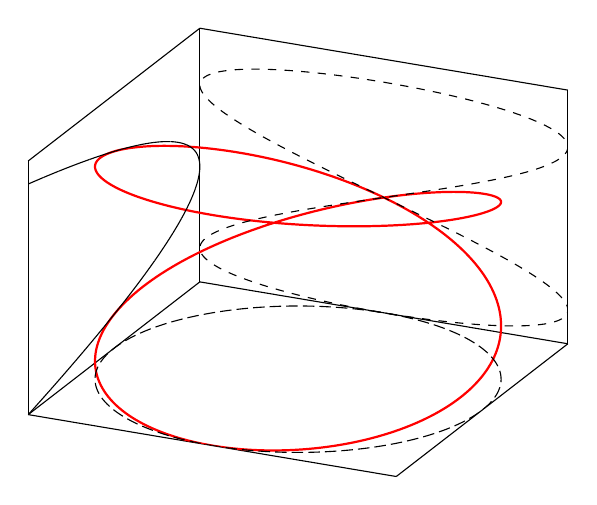
\begin{tikzpicture}
      \begin{axis}[
        xtick   = \empty,
        ytick   = \empty,
        ztick   = \empty,
        xmin    = -1,
        ymax    = 2,
        zmin    = -2,
      ]
      \addplot3+ [
        domain     = 0:360,
        samples    = 400,
        samples y  = 0,
        mark       = none,
        thick,
        red,
      ]
      ( {sin(2*x)}, {2*(sin(x))^2}, {2*cos(x)} );
      \addplot3+ [
        domain     = 0:360,
        samples    = 400,
        samples y  = 0,
        mark       = none,
        dashed,
        black,
      ]
      ( {-1}, {2*(sin(x))^2}, {2*cos(x)} );
      \addplot3+ [
        domain     = 0:360,
        samples    = 400,
        samples y  = 0,
        mark       = none,
        dashed,
        black,
      ]
      ( {sin(2*x)}, {2}, {2*cos(x)} );
      \addplot3+ [
        domain     = 0:360,
        samples    = 400,
        samples y  = 0,
        mark       = none,
        dashed,
        black,
      ]
      ( {sin(2*x)}, {2*(sin(x))^2}, {-2} );
      \end{axis}
    \end{tikzpicture}
    \end{center}
    
    \item $\vec r(t) = (\sin 2t, 2\sin^2 t, 2\cos t) = (\sin 2t, 1 - \cos 2t, 2\cos t)$. Dessa forma,
    \begin{align*}
        \dot{\vec r}(t) = (2\cos 2t, 2 \sin 2t, -2 \sin t).
    \end{align*}
    Sabemos que as funções seno e cosseno nunca se anulam simultaneamente, logo $\dot{\vec r}(t) \neq (0,0,0)~\forall t\in[0,2 \pi]$, o que mostra que a curva é regular.
    
    \item A projeção de $\dot{\vec r}(t)$ sobre o plano $z = 0$ é dada por $(2\cos 2t, 2 \sin 2t, 0)$ e cuja norma euclidiana é 2.
  \end{enumerate}
\end{solution}

% 2.8 % % % % % % % % % % % % % % % % % % % % %
% \setcounter{question}{5}
\question{
Seja $\vec r \, : \, \R \to \R^3$ dada por $\vec r(t) = \left( \frac{4}{5} \cos 5t, -\sin 5t, -\frac{3}{5} \cos 5t \right)$. Mostre que o traço de $\vec r$ é uma circunferência. Determine seu centro, seu raio e o plano que o contém.
}

\begin{solution}
    O versor tangente, normal e binormal da trajetória são, respectivamente,
    \begin{align*}
        \hat{T}(t) &= \frac{\dot{\vec r}(t)}{|\dot{\vec r}(t)|}
            = \left\{-\tfrac{4}{5} \sin (5 t),-\cos (5 t),\tfrac{3}{5} \sin (5 t)\right\} , \\
        \hat{N}(t) &= \frac{\dot{\hat T}(t)}{|\dot{\hat T}(t)|} = \left\{-\tfrac{4}{5} \cos (5 t),\sin (5 t),\tfrac{3}{5} \cos (5 t)\right\}, \\
        \hat{B}(t) &= \hat{T} \times \hat{N} = \left\{-\frac{3}{5},~0,~-\frac{4}{5}\right\}.
    \end{align*}
    Para mostrar que é uma circunferência, temos que constatar que a curvatura é constante não-nula (raio constante) e a torção é nula (permance em um plano). De fato,
    \begin{align*}
        \kappa(t) &= \frac{|\dot{\hat T}(t)|}{|\dot{\vec r}(t)|} = 1,\\
        \tau(t) &= - \hat{N}(t)\cdot\dot{\hat{B}}(t) = 0.
    \end{align*}
    Sabemos que o raio é o inverso da curvatura, ou seja, o raio é 1.
    
    O plano que contém a circunferência tem como vetor normal o versor binormal $\hat{B}$. Assim, a equação do plano deve satisfazer
    \begin{align*}
        \hat{B}\cdot\big((x,y,z)-(0,-1,0)\big) = 0 
            ~\Leftrightarrow~ 3x + 4z = 0,
    \end{align*}
    onde $(0,-1,0) = \vec{r}(\pi/10)$ é um ponto da circunferência.
    
    O centro da circunferência está na origem.
\end{solution}

% 2.9 % % % % % % % % % % % % % % % % % % % % %
% \setcounter{question}{11}
\question{
Seja $\vec r \, : \, \R \to \R^3$ dada por $\vec r(t) = (\cos t, \sin t, 1 - \sin t)$.
  \begin{enumerate}[label=(\alph*)]
    \item Mostre que o traço de $\vec r$ está contida no cilindro $x^2 + y^2 = 1$.
    \item Obtenha o Triedro de Frenet, a curvatura e a torção de $\vec r$.
    \item Mostre que $\vec r$ é uma curva plana e determine o plano que a contém. Por que isto implica que $\vec r$ é uma elipse?
    \item Em que pontos de $\vec r$ a curvatura é máxima? Em que pontos ela é mínima? Interperte geometricamente.
  \end{enumerate}
}
\begin{solution}
  \begin{enumerate}[label=(\alph*)]
    \item De fato, $\cos^2 t + \sin^2 t = 1$, portanto, $\vec r$ está contida nesse cilindro.
    
    \item ~\vspace{-5mm}
    \begin{align*}
        \hat{T}(t) 
            &= \frac{\dot{\vec r}(t)}{|\dot{\vec r}(t)|}
            = \frac{\{-\sin (t),\cos (t),-\cos (t)\}}{\sqrt{1+\cos^2(t)}} , \\
        \hat{N}(t) 
            &= \frac{\dot{\hat T}(t)}{|\dot{\hat T}(t)|}
            = \frac{\{-2\cos(t), -\sin(t), \sin(t)\}}{\sqrt{2(1+\cos^2(t))}}, \\
        \hat{B}(t) 
            &= \hat{T} \times \hat{N} = \frac{\{0,1,1\}}{\sqrt{2}},\\
        \kappa(t)
            &= \frac{|\dot{\vec r}(t) \times \ddot{\vec r}(t)|}{|\dot{\vec r}(t)|^3}
            = \frac{\sqrt{2}}{(1+\cos^2(t))^{3/2}},\\
        \tau(t) 
            &= - \hat{N}(t)\cdot\dot{\hat{B}}(t) = 0.
    \end{align*}
    
    
    \item A curva $\vec r$ é plana, pois a torção $\tau(t)=0~\forall t\in\R$.
    
    O plano que contém a curva tem como vetor normal o versor binormal $\hat{B}$. Assim, a equação do plano deve satisfazer
    \begin{align*}
        \hat{B}\cdot\big((x,y,z)-(1,0,1)\big) = 0 
            ~\Leftrightarrow~ y + z = 1,
    \end{align*}
    onde $(1,0,1) = \vec{r}(0)$ é um ponto da curva.
    
    Isso implica que $\vec r$ é uma elipse, pois é a interseção de um plano com um cilindro.
    
    \item A curvatura $\kappa(t)$ é máxima quando $\cos(t) = 0$, ou seja, em $\vec{r}(t=\pi/2) = (0,1,1)$ e $\vec{r}(t=3\pi/2) = (0,-1,2)$, que são os pontos que cruzam com o eixo maior da elipse.
    
    A curvatura $\kappa(t)$ é mínima quando $\cos(t) = \pm1$, ou seja, em $\vec{r}(t=0) = (1,0,1)$ e $\vec{r}(t=\pi) = (-1,0,1)$, que são os pontos que cruzam com o eixo menor da elipse.
  \end{enumerate}
\end{solution}

\end{questions}
